\PassOptionsToPackage{unicode=true}{hyperref} % options for packages loaded elsewhere
\PassOptionsToPackage{hyphens}{url}
%
\documentclass[
  ignorenonframetext,
]{beamer}
\usepackage{pgfpages}
\setbeamertemplate{caption}[numbered]
\setbeamertemplate{caption label separator}{: }
\setbeamercolor{caption name}{fg=normal text.fg}
\beamertemplatenavigationsymbolsempty
% Prevent slide breaks in the middle of a paragraph:
\widowpenalties 1 10000
\raggedbottom
\setbeamertemplate{part page}{
  \centering
  \begin{beamercolorbox}[sep=16pt,center]{part title}
    \usebeamerfont{part title}\insertpart\par
  \end{beamercolorbox}
}
\setbeamertemplate{section page}{
  \centering
  \begin{beamercolorbox}[sep=12pt,center]{part title}
    \usebeamerfont{section title}\insertsection\par
  \end{beamercolorbox}
}
\setbeamertemplate{subsection page}{
  \centering
  \begin{beamercolorbox}[sep=8pt,center]{part title}
    \usebeamerfont{subsection title}\insertsubsection\par
  \end{beamercolorbox}
}
\AtBeginPart{
  \frame{\partpage}
}
\AtBeginSection{
  \ifbibliography
  \else
    \frame{\sectionpage}
  \fi
}
\AtBeginSubsection{
  \frame{\subsectionpage}
}
\usepackage{lmodern}
\usepackage{amssymb,amsmath}
\usepackage{ifxetex,ifluatex}
\ifnum 0\ifxetex 1\fi\ifluatex 1\fi=0 % if pdftex
  \usepackage[T1]{fontenc}
  \usepackage[utf8]{inputenc}
  \usepackage{textcomp} % provides euro and other symbols
\else % if luatex or xelatex
  \usepackage{unicode-math}
  \defaultfontfeatures{Scale=MatchLowercase}
  \defaultfontfeatures[\rmfamily]{Ligatures=TeX,Scale=1}
\fi
% use upquote if available, for straight quotes in verbatim environments
\IfFileExists{upquote.sty}{\usepackage{upquote}}{}
\IfFileExists{microtype.sty}{% use microtype if available
  \usepackage[]{microtype}
  \UseMicrotypeSet[protrusion]{basicmath} % disable protrusion for tt fonts
}{}
\makeatletter
\@ifundefined{KOMAClassName}{% if non-KOMA class
  \IfFileExists{parskip.sty}{%
    \usepackage{parskip}
  }{% else
    \setlength{\parindent}{0pt}
    \setlength{\parskip}{6pt plus 2pt minus 1pt}}
}{% if KOMA class
  \KOMAoptions{parskip=half}}
\makeatother
\usepackage{xcolor}
\IfFileExists{xurl.sty}{\usepackage{xurl}}{} % add URL line breaks if available
\IfFileExists{bookmark.sty}{\usepackage{bookmark}}{\usepackage{hyperref}}
\hypersetup{
  pdftitle={4 - Computational approaches},
  pdfborder={0 0 0},
  breaklinks=true}
\urlstyle{same}  % don't use monospace font for urls
\newif\ifbibliography
\usepackage{color}
\usepackage{fancyvrb}
\newcommand{\VerbBar}{|}
\newcommand{\VERB}{\Verb[commandchars=\\\{\}]}
\DefineVerbatimEnvironment{Highlighting}{Verbatim}{commandchars=\\\{\}}
% Add ',fontsize=\small' for more characters per line
\usepackage{framed}
\definecolor{shadecolor}{RGB}{248,248,248}
\newenvironment{Shaded}{\begin{snugshade}}{\end{snugshade}}
\newcommand{\AlertTok}[1]{\textcolor[rgb]{0.94,0.16,0.16}{#1}}
\newcommand{\AnnotationTok}[1]{\textcolor[rgb]{0.56,0.35,0.01}{\textbf{\textit{#1}}}}
\newcommand{\AttributeTok}[1]{\textcolor[rgb]{0.77,0.63,0.00}{#1}}
\newcommand{\BaseNTok}[1]{\textcolor[rgb]{0.00,0.00,0.81}{#1}}
\newcommand{\BuiltInTok}[1]{#1}
\newcommand{\CharTok}[1]{\textcolor[rgb]{0.31,0.60,0.02}{#1}}
\newcommand{\CommentTok}[1]{\textcolor[rgb]{0.56,0.35,0.01}{\textit{#1}}}
\newcommand{\CommentVarTok}[1]{\textcolor[rgb]{0.56,0.35,0.01}{\textbf{\textit{#1}}}}
\newcommand{\ConstantTok}[1]{\textcolor[rgb]{0.00,0.00,0.00}{#1}}
\newcommand{\ControlFlowTok}[1]{\textcolor[rgb]{0.13,0.29,0.53}{\textbf{#1}}}
\newcommand{\DataTypeTok}[1]{\textcolor[rgb]{0.13,0.29,0.53}{#1}}
\newcommand{\DecValTok}[1]{\textcolor[rgb]{0.00,0.00,0.81}{#1}}
\newcommand{\DocumentationTok}[1]{\textcolor[rgb]{0.56,0.35,0.01}{\textbf{\textit{#1}}}}
\newcommand{\ErrorTok}[1]{\textcolor[rgb]{0.64,0.00,0.00}{\textbf{#1}}}
\newcommand{\ExtensionTok}[1]{#1}
\newcommand{\FloatTok}[1]{\textcolor[rgb]{0.00,0.00,0.81}{#1}}
\newcommand{\FunctionTok}[1]{\textcolor[rgb]{0.00,0.00,0.00}{#1}}
\newcommand{\ImportTok}[1]{#1}
\newcommand{\InformationTok}[1]{\textcolor[rgb]{0.56,0.35,0.01}{\textbf{\textit{#1}}}}
\newcommand{\KeywordTok}[1]{\textcolor[rgb]{0.13,0.29,0.53}{\textbf{#1}}}
\newcommand{\NormalTok}[1]{#1}
\newcommand{\OperatorTok}[1]{\textcolor[rgb]{0.81,0.36,0.00}{\textbf{#1}}}
\newcommand{\OtherTok}[1]{\textcolor[rgb]{0.56,0.35,0.01}{#1}}
\newcommand{\PreprocessorTok}[1]{\textcolor[rgb]{0.56,0.35,0.01}{\textit{#1}}}
\newcommand{\RegionMarkerTok}[1]{#1}
\newcommand{\SpecialCharTok}[1]{\textcolor[rgb]{0.00,0.00,0.00}{#1}}
\newcommand{\SpecialStringTok}[1]{\textcolor[rgb]{0.31,0.60,0.02}{#1}}
\newcommand{\StringTok}[1]{\textcolor[rgb]{0.31,0.60,0.02}{#1}}
\newcommand{\VariableTok}[1]{\textcolor[rgb]{0.00,0.00,0.00}{#1}}
\newcommand{\VerbatimStringTok}[1]{\textcolor[rgb]{0.31,0.60,0.02}{#1}}
\newcommand{\WarningTok}[1]{\textcolor[rgb]{0.56,0.35,0.01}{\textbf{\textit{#1}}}}
\usepackage{longtable,booktabs}
\usepackage{caption}
% These lines are needed to make table captions work with longtable:
\makeatletter
\def\fnum@table{\tablename~\thetable}
\makeatother
\usepackage{graphicx,grffile}
\makeatletter
\def\maxwidth{\ifdim\Gin@nat@width>\linewidth\linewidth\else\Gin@nat@width\fi}
\def\maxheight{\ifdim\Gin@nat@height>\textheight\textheight\else\Gin@nat@height\fi}
\makeatother
% Scale images if necessary, so that they will not overflow the page
% margins by default, and it is still possible to overwrite the defaults
% using explicit options in \includegraphics[width, height, ...]{}
\setkeys{Gin}{width=\maxwidth,height=\maxheight,keepaspectratio}
\setlength{\emergencystretch}{3em}  % prevent overfull lines
\providecommand{\tightlist}{%
  \setlength{\itemsep}{0pt}\setlength{\parskip}{0pt}}
\setcounter{secnumdepth}{-2}

% set default figure placement to htbp
\makeatletter
\def\fps@figure{htbp}
\makeatother

\titlegraphic{\centering 
\includegraphics[width=5cm]{mpidr_logo_dag.pdf}}
\setbeamertemplate{navigation symbols}{} 
\setbeamertemplate{footline}[frame number]

\title{4 - Computational approaches}
\author{Diego Alburez-Gutierrez\\
MPIDR\\
European Doctoral School of Demography 2019-20}
\date{02/04/2020}

\begin{document}
\frame{\titlepage}

\begin{frame}{Agenda}
\protect\hypertarget{agenda}{}

\begin{enumerate}
\tightlist
\item
  Q\&A
\item
  Demographic micro simulation
\item
  Example 1: Impact of the HIV/AIDS epidemic on kinship resources
\item
  Example 2: Projecting older adults without kin
\item
  Discussion
\end{enumerate}

\end{frame}

\begin{frame}{Q\&A}
\protect\hypertarget{qa}{}

\begin{itemize}
\tightlist
\item
  Previous days
\item
  Questions about final assignment
\item
  Other?
\end{itemize}

\end{frame}

\begin{frame}{Demographic micro-simulation}
\protect\hypertarget{demographic-micro-simulation}{}

\begin{itemize}
\tightlist
\item
  Model individual-level demographic behaviour applying set of rules
\item
  Make up data where unavailable
\item
  Science: compare to independent method
\item
  Different alternatives:

  \begin{itemize}
  \tightlist
  \item
    SOCSIM
  \item
    CAMSIM
  \item
    NetLogo (Agent-based modelling)
  \item
    R/python
  \end{itemize}
\end{itemize}

\tiny Grow, A and Van Bavel, J. 2018. Agent-Based Modeling of Family
Formation and Dissolution. In R. Schoen (Ed.), Analytical Family
Demography (pp.~125-156). Springer Series on Demographic Methods and
Population Analysis, (Vol. 47), Cham: Springer International Publishing.

\end{frame}

\begin{frame}{Creating digital populations with SOCSIM}
\protect\hypertarget{creating-digital-populations-with-socsim}{}

\begin{itemize}
\tightlist
\item
  A stochastic micro-simulation platform, 1970s at UC Berkeley
\item
  Starting with an initial population, applies age-specific demographic
  rates
\item
  Creates kinship structure similar to a full genealogy
\item
  Now maintained at the MPIDR!
\end{itemize}

\tiny Mason, C. (2016). SOCSIM Oversimplified. UC Berkeley.
\url{https://lab.demog.berkeley.edu/socsim/CurrentDocs/socsimOversimplified.pdf}

\end{frame}

\begin{frame}{SOCSIM}
\protect\hypertarget{socsim}{}

\begin{figure}
\centering
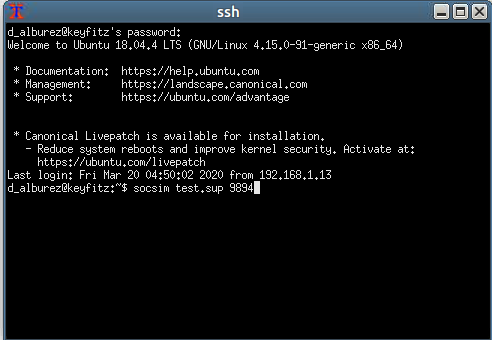
\includegraphics[width=3.125in,height=\textheight]{resources/socsim.PNG}
\caption{What microsimulation actually looks like}
\end{figure}

\end{frame}

\begin{frame}[fragile]{A SOCSIM micro-simulation of Sweden (1603-2160)}
\protect\hypertarget{a-socsim-micro-simulation-of-sweden-1603-2160}{}

\begin{Shaded}
\begin{Highlighting}[]
\CommentTok{# Read sample Familinx data using data.table}
\KeywordTok{read.csv}\NormalTok{(}\StringTok{"../../Assignment/Data/sweden_socsim.csv"}\NormalTok{) }\OperatorTok\StringTok{ }
\StringTok{  }\KeywordTok{slice}\NormalTok{(}\DecValTok{1}\OperatorTok{:}\DecValTok{4}\NormalTok{) }\OperatorTok\StringTok{ }
\StringTok{  }\KeywordTok{kable}\NormalTok{()}
\end{Highlighting}
\end{Shaded}

\begin{longtable}[]{@{}rrrrr@{}}
\toprule
profileid & father & mother & birth\_year & death\_year\tabularnewline
\midrule
\endhead
10000 & 2152 & 2390 & 1703 & 1705\tabularnewline
10001 & 0 & 4343 & 1703 & 1707\tabularnewline
10002 & 4593 & 5190 & 1703 & 1773\tabularnewline
10003 & 0 & 3252 & 1703 & 1703\tabularnewline
\bottomrule
\end{longtable}

\tiny Zagheni, E. 2017. The Demographic Foundations of the Lived
Experience of Kin Death. Working paper.

\end{frame}

\begin{frame}{Historical and projected demographic processes}
\protect\hypertarget{historical-and-projected-demographic-processes}{}

\begin{figure}
\centering
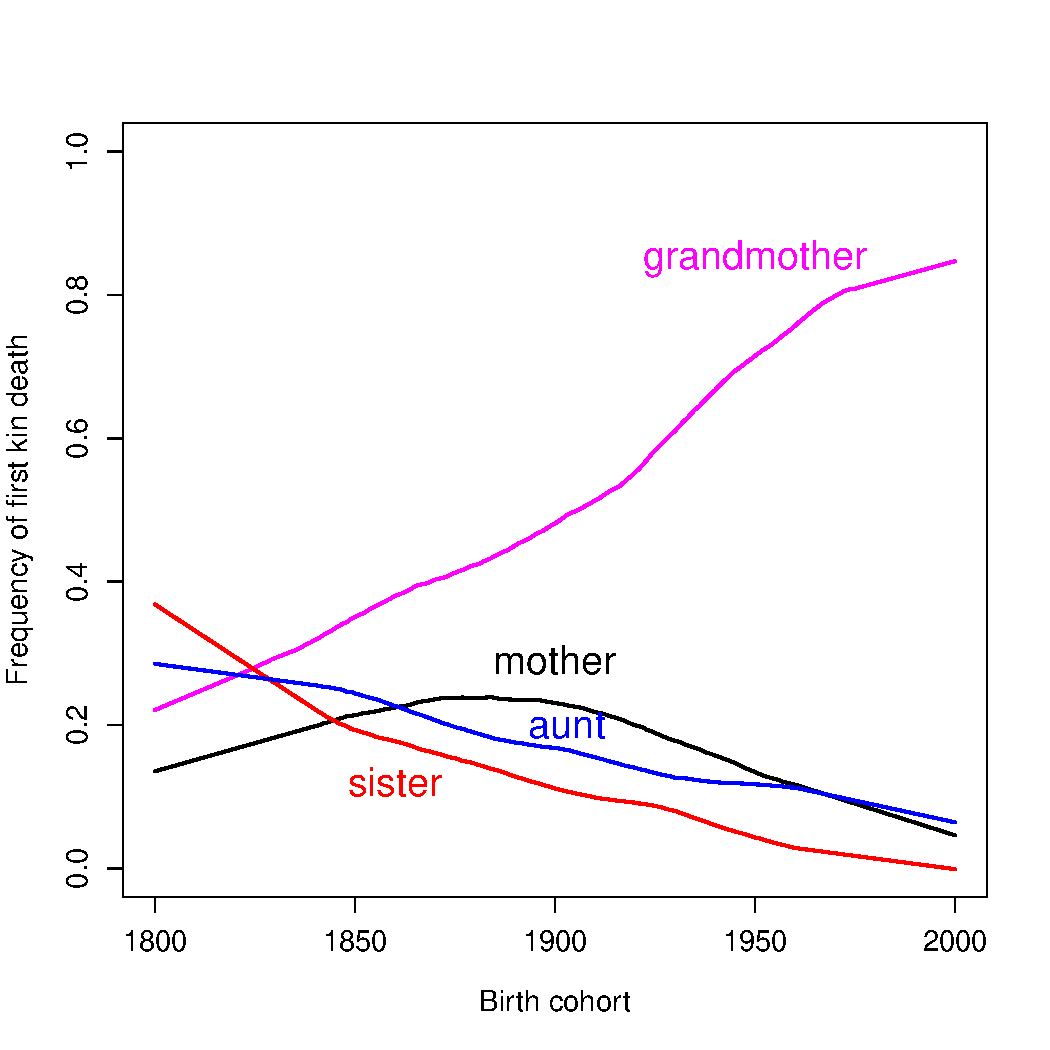
\includegraphics[width=3.125in,height=\textheight]{resources/type_kin_death}
\caption{Frequency of different types of kin death, Sweden (SOCSIM)}
\end{figure}

\tiny Zagheni, E. 2017. The Demographic Foundations of the Lived
Experience of Kin Death. Working paper.

\end{frame}

\begin{frame}{Question time!}
\protect\hypertarget{question-time}{}


\includegraphics[width=0.41667in,height=\textheight]{resources/light.png}

\end{frame}

\begin{frame}[fragile]{Some magic sampling\ldots{}}
\protect\hypertarget{some-magic-sampling}{}


\includegraphics[width=0.3125in,height=\textheight]{resources/ball.png}

\begin{verbatim}
## [1] "Alexander" "Madalina"  "Octavio"
\end{verbatim}

\end{frame}

\hypertarget{example-1-impact-of-the-hivaids-epidemic-on-kinship-resources}{%
\section{Example 1: Impact of the HIV/AIDS epidemic on kinship
resources}\label{example-1-impact-of-the-hivaids-epidemic-on-kinship-resources}}

\begin{frame}{Research at a glance}
\protect\hypertarget{research-at-a-glance}{}

\begin{itemize}
\tightlist
\item
  RQ: estimate and project probabilities of orphanhood and evolution of
  kinship structure in Zimbabwe in context of HIV/AIDS epidemic
  (1980-2050)
\item
  Data: SOCSIM, with rates from UN WPP, Demographic and Health Surveys,
  World Fertility and Marriage Database, UN HIV infection rates
\item
  Findings:

  \begin{itemize}
  \tightlist
  \item
    increase in double orphans with no living grandparents
  \item
    shift of responsibilities to aunts and uncles
  \end{itemize}
\end{itemize}

\tiny\{Zagheni, E. 2011. The impact of the HIV/AIDS epidemic on kinship
resources for orphans in Zimbabwe, Population and Development Review
74(4), 761-783.\}

\end{frame}

\begin{frame}{Double-orphans and double-orphans without grandparents}
\protect\hypertarget{double-orphans-and-double-orphans-without-grandparents}{}

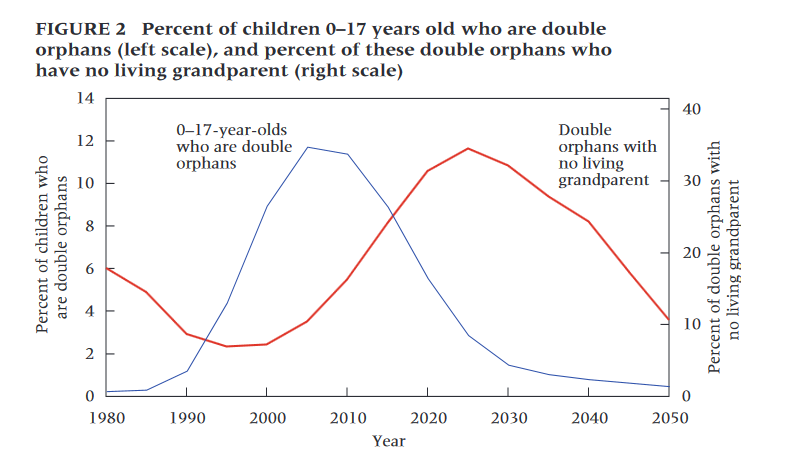
\includegraphics[width=3.64583in,height=\textheight]{resources/zagheni_orphans.PNG}

\tiny\{Zagheni, E. 2011. The impact of the HIV/AIDS epidemic on kinship
resources for orphans in Zimbabwe, Population and Development Review
74(4), 761-783.\}

\end{frame}

\begin{frame}{Percent of double orphans}
\protect\hypertarget{percent-of-double-orphans}{}

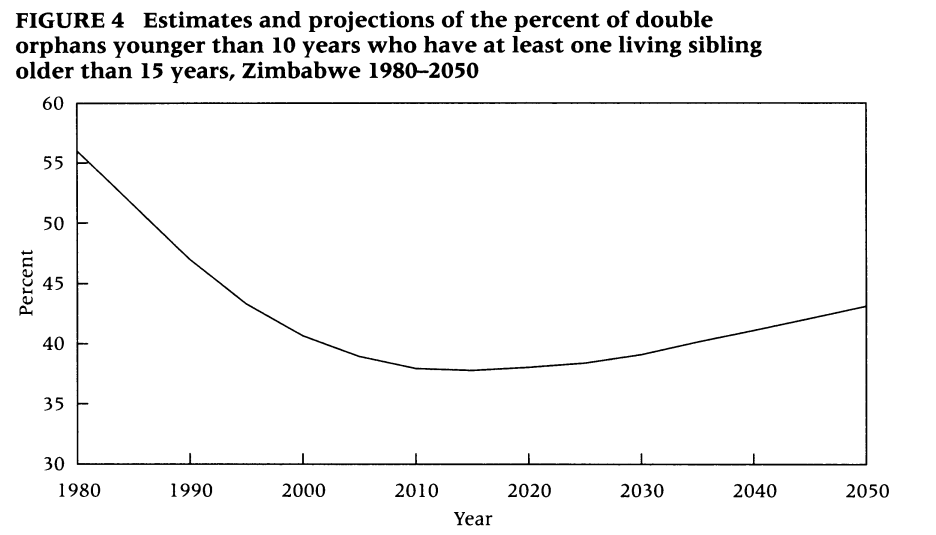
\includegraphics[width=3.64583in,height=\textheight]{resources/zag4.PNG}

\tiny\{Zagheni, E. 2011. The impact of the HIV/AIDS epidemic on kinship
resources for orphans in Zimbabwe, Population and Development Review
74(4), 761-783.\}

\end{frame}

\begin{frame}{Availability of aunts and uncles}
\protect\hypertarget{availability-of-aunts-and-uncles}{}

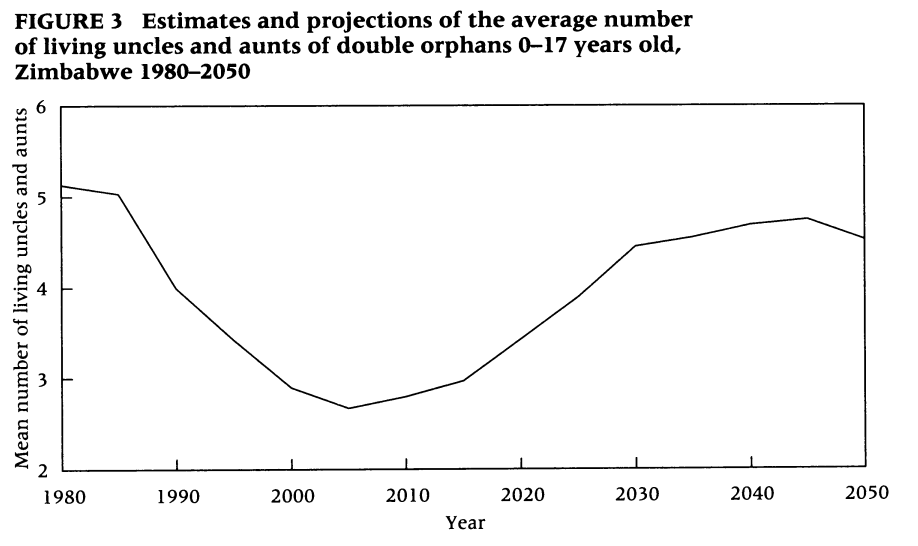
\includegraphics[width=3.64583in,height=\textheight]{resources/zag3.PNG}

\tiny\{Zagheni, E. 2011. The impact of the HIV/AIDS epidemic on kinship
resources for orphans in Zimbabwe, Population and Development Review
74(4), 761-783.\}

\end{frame}

\hypertarget{example-2-projecting-older-adults-without-kin}{%
\section{Example 2: Projecting older adults without
kin}\label{example-2-projecting-older-adults-without-kin}}

\begin{frame}{Research at a glance}
\protect\hypertarget{research-at-a-glance-1}{}

\begin{itemize}
\tightlist
\item
  RQ: Examine the changing population of kinless individuals in American
  society over the coming decades
\item
  Data: Rates from US census, Human Fertility Database, official
  statistics
\item
  Findings:

  \begin{itemize}
  \tightlist
  \item
    impending increase of kinless older adults, especially amongst Black
  \item
    Declines in marriage, one-child families, mortality
  \end{itemize}
\end{itemize}

\tiny Verdery, A.M. and Margolis, R. (2017). Projections of white and
black older adults without living kin in the United States, 2015 to
2060. Proceedings of the National Academy of Sciences
114(42):11109--11114.

\end{frame}

\begin{frame}{Data sources}
\protect\hypertarget{data-sources}{}

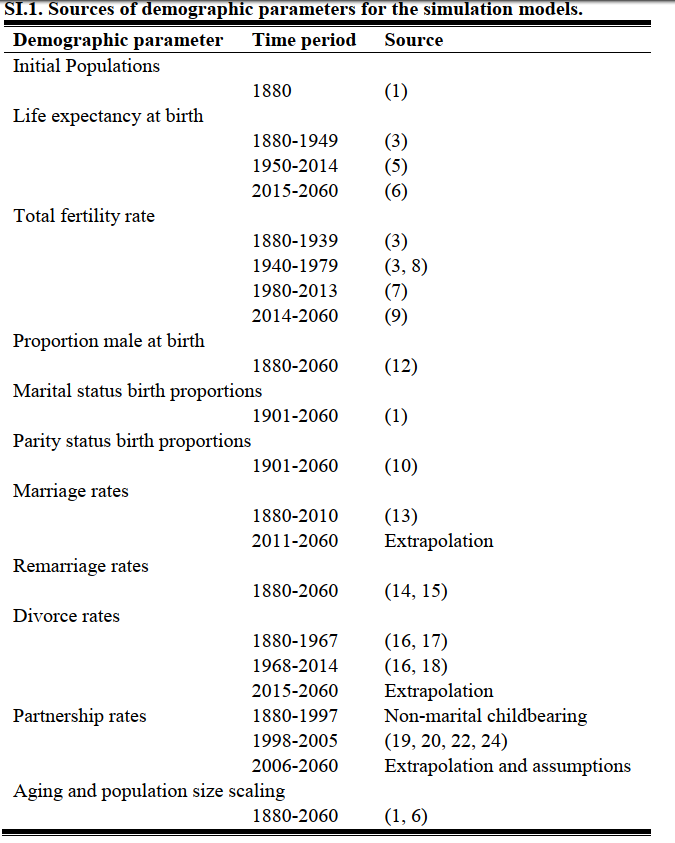
\includegraphics[width=2.60417in,height=\textheight]{resources/verdery_sources.PNG}

\end{frame}

\begin{frame}{Sanity checks: comparing to ground-truth}
\protect\hypertarget{sanity-checks-comparing-to-ground-truth}{}

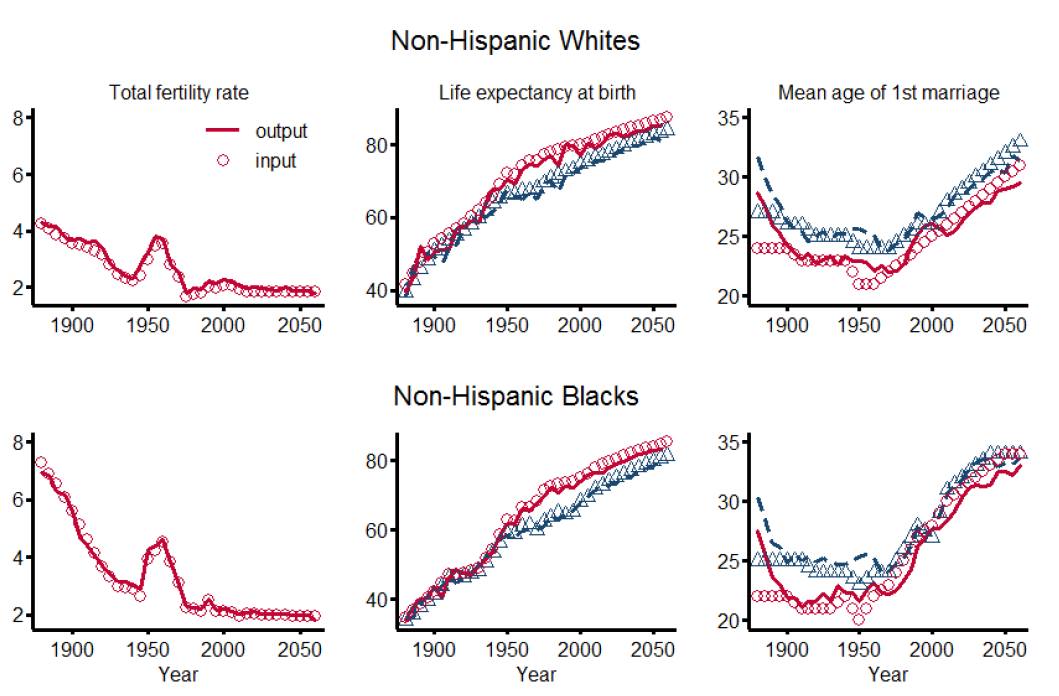
\includegraphics[width=3.64583in,height=\textheight]{resources/verdery_rates.PNG}

Key rates, historical and projected changes over time and simulated
outcomes, 1880- 2060.

\tiny Verdery, A.M. and Margolis, R. (2017). SI Appendix. Projections of
white and black older adults without living kin in the United States,
2015 to 2060. Proceedings of the National Academy of Sciences
114(42):11109--11114.

\end{frame}

\begin{frame}{Kinlesness by gender and ethnicity in the US}
\protect\hypertarget{kinlesness-by-gender-and-ethnicity-in-the-us}{}

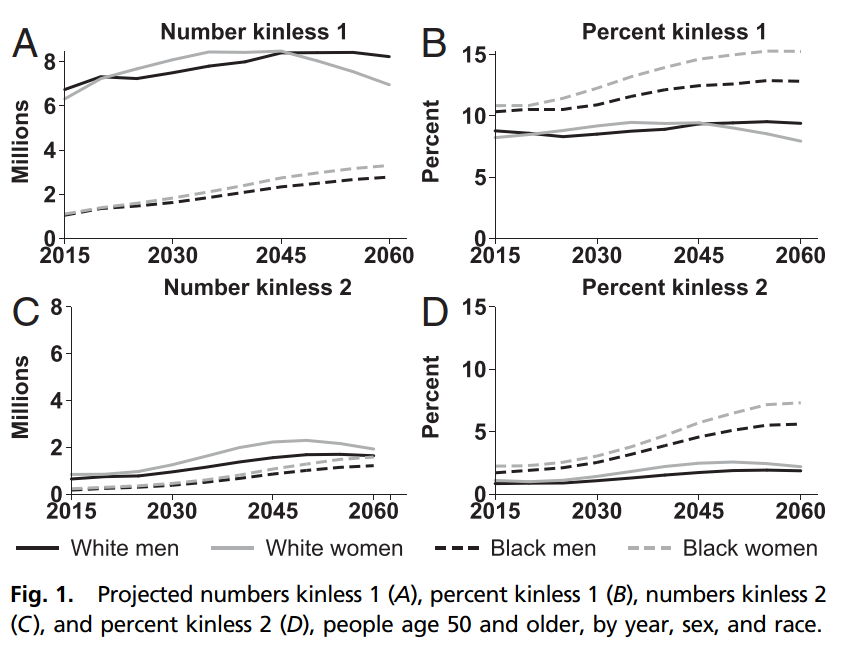
\includegraphics[width=3.64583in,height=\textheight]{resources/verdery.PNG}

\tiny Verdery, A.M. and Margolis, R. (2017). Projections of white and
black older adults without living kin in the United States, 2015 to
2060. Proceedings of the National Academy of Sciences
114(42):11109--11114.

\end{frame}

\begin{frame}{Beyond description: looking at mechanisms}
\protect\hypertarget{beyond-description-looking-at-mechanisms}{}

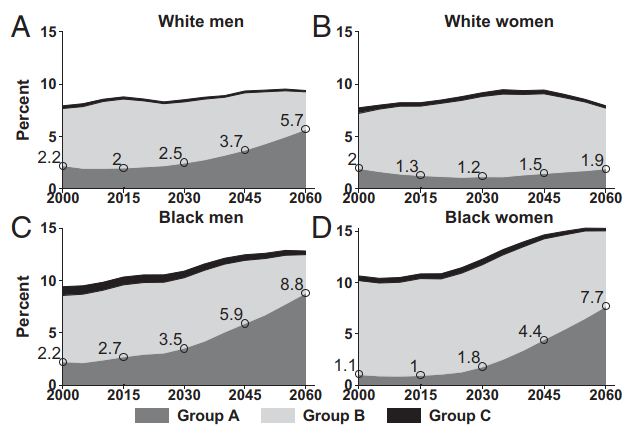
\includegraphics[width=3.64583in,height=\textheight]{resources/verdery_mechanisms.PNG}

\tiny Verdery, A.M. and Margolis, R. (2017). Projections of white and
black older adults without living kin in the United States, 2015 to
2060. Proceedings of the National Academy of Sciences
114(42):11109--11114.

\end{frame}

\hypertarget{discussion}{%
\section{Discussion}\label{discussion}}

\begin{frame}{Strengths and weaknesses of simulated data}
\protect\hypertarget{strengths-and-weaknesses-of-simulated-data}{}

\begin{itemize}
\tightlist
\item
  Impact of the HIV/AIDS epidemic

  \begin{itemize}
  \tightlist
  \item
    Pro: No alternative data source
  \item
    Pro: accounts for clustering of mortality
  \item
    Con: comparison to ground-truth?
  \item
    Con: high uncertainty of projected rates used as input in this
    context
  \end{itemize}
\item
  Projecting older adults without kin

  \begin{itemize}
  \tightlist
  \item
    Pro: Projection based on real rates
  \item
    Pro: unpacks demographic dynamics leading to outcome
  \item
    Con: model assumptions about marriage market
  \item
    Con: comparison to ground-truth?
  \item
    Con: does not account for future mortality shocks
  \end{itemize}
\end{itemize}

\end{frame}

\begin{frame}{When should we use real and simulated populations?}
\protect\hypertarget{when-should-we-use-real-and-simulated-populations}{}

\begin{itemize}
\tightlist
\item
  Use real data whenever possible
\item
  Improve the interval validity of simulations

  \begin{itemize}
  \tightlist
  \item
    Calibration
  \item
    Methodological triangulation
  \item
    Comparing simulations to ground-truth
  \end{itemize}
\end{itemize}

\end{frame}

\begin{frame}[fragile]{A SOCSIM micro-simulation of Sweden (1603-2160)}
\protect\hypertarget{a-socsim-micro-simulation-of-sweden-1603-2160-1}{}

\begin{Shaded}
\begin{Highlighting}[]
\CommentTok{# Read sample Familinx data using data.table}
\KeywordTok{read.csv}\NormalTok{(}\StringTok{"../../Assignment/Data/sweden_socsim.csv"}\NormalTok{) }\OperatorTok\StringTok{ }
\StringTok{  }\KeywordTok{slice}\NormalTok{(}\DecValTok{1}\OperatorTok{:}\DecValTok{4}\NormalTok{) }\OperatorTok\StringTok{ }
\StringTok{  }\KeywordTok{kable}\NormalTok{()}
\end{Highlighting}
\end{Shaded}

\begin{longtable}[]{@{}rrrrr@{}}
\toprule
profileid & father & mother & birth\_year & death\_year\tabularnewline
\midrule
\endhead
10000 & 2152 & 2390 & 1703 & 1705\tabularnewline
10001 & 0 & 4343 & 1703 & 1707\tabularnewline
10002 & 4593 & 5190 & 1703 & 1773\tabularnewline
10003 & 0 & 3252 & 1703 & 1703\tabularnewline
\bottomrule
\end{longtable}

\end{frame}

\begin{frame}{Where did this SOCSIM simulation come from?}
\protect\hypertarget{where-did-this-socsim-simulation-come-from}{}

\begin{enumerate}
\tightlist
\item
  Initial population
\item
  Age-speficid fertility rates
\item
  Age-speficid mortality rates
\item
  Marriage transition rates
\item
  Model for marriage market
\item
  Other parameters (inheritance of fertility, etc.)
\end{enumerate}

\end{frame}

\begin{frame}{A quick example of such a comparison}
\protect\hypertarget{a-quick-example-of-such-a-comparison}{}

\begin{itemize}
\tightlist
\item
  Cumulative number of child deaths for a woman surviving to a given age

  \begin{itemize}
  \tightlist
  \item
    Estimate from SOCISM-generated genealogy
  \item
    Estimate formally:
  \end{itemize}
\end{itemize}

\begin{equation}
\underbrace{CD_{(a,c, p)}}_{\text{Child deaths}}= \underbrace{\sum_{x=15}^{x=a} {_1F_{(x,c,p)}}}_{\text{Children born}}-\underbrace{\sum_{x=15}^{x=a} {_1F_{(x,c,p)}} l_{(a-x,c+x,p)}}_{\text{Children surviving or } CS_{(a,c,p)} }
\end{equation}

\end{frame}

\begin{frame}{Methodological triangulation: model and formal estimates}
\protect\hypertarget{methodological-triangulation-model-and-formal-estimates}{}

\begin{figure}
\centering
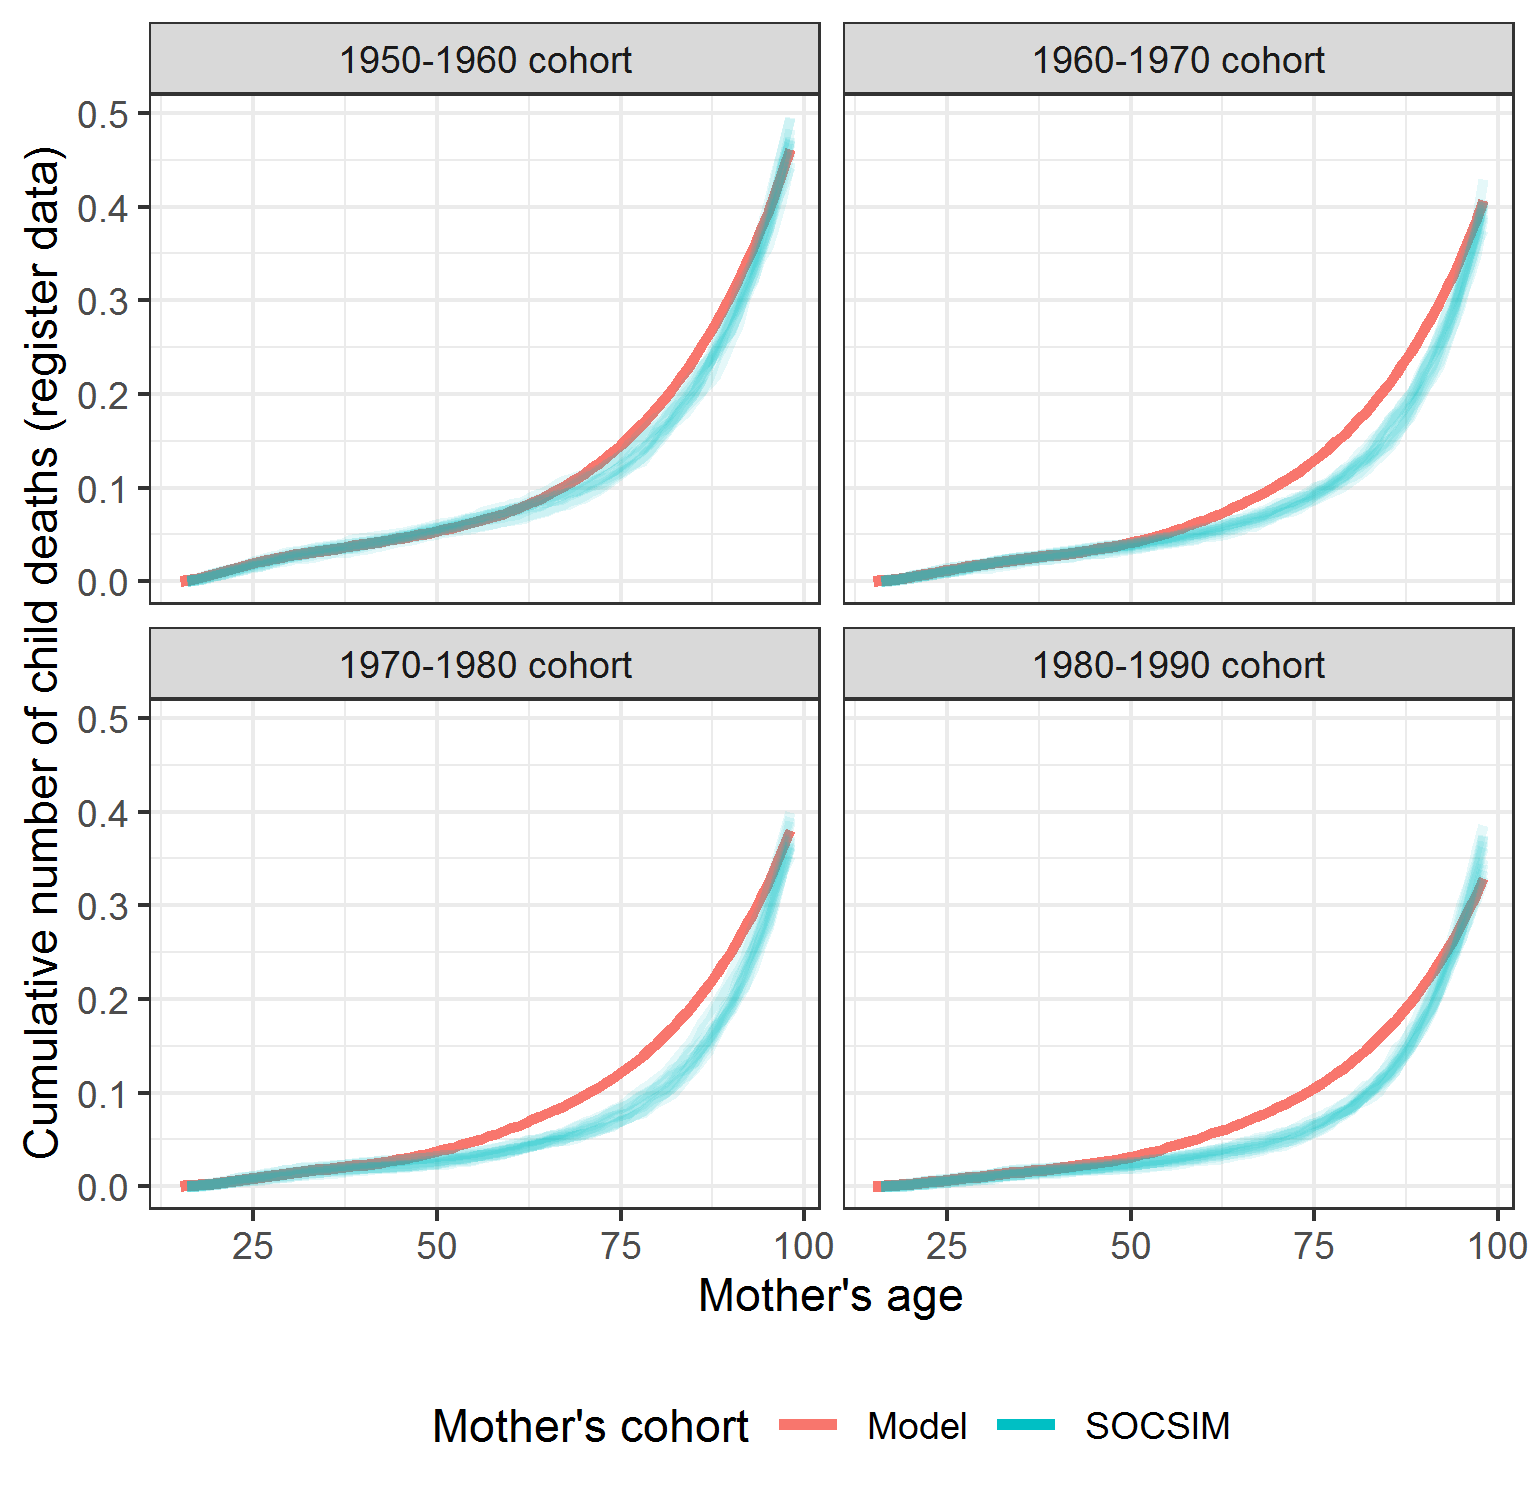
\includegraphics[width=3.64583in,height=\textheight]{resources/child_loss_decade}
\caption{Expected number of child deaths}
\end{figure}

\end{frame}

\begin{frame}{More validation: Compare to `gold-standard' data}
\protect\hypertarget{more-validation-compare-to-gold-standard-data}{}

\begin{figure}
\centering
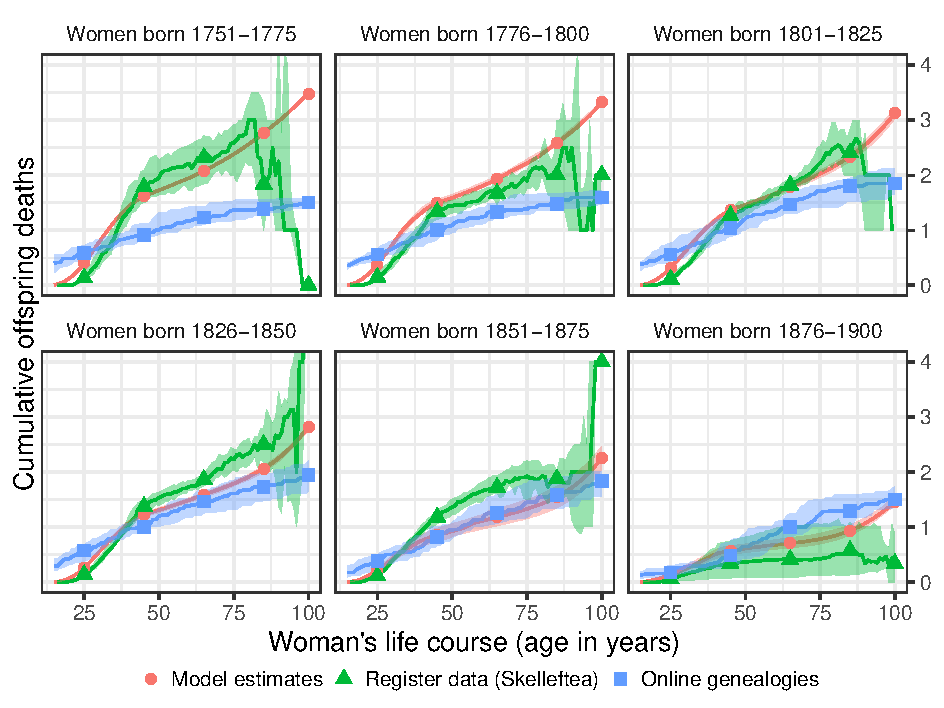
\includegraphics[width=3.64583in,height=\textheight]{resources/comparative}
\caption{Expected number of child deaths}
\end{figure}

\end{frame}

\begin{frame}{Another example: sandwichness}
\protect\hypertarget{another-example-sandwichness}{}

\begin{itemize}
\tightlist
\item
  `Sandwiched' between having a young child and a parent close to death
\item
  Double care responsibility
\item
  Change over time
\end{itemize}

\begin{equation*}
S(a,c) = \underbrace{  (1 -  \prod_{x=1}^{5} 1 - F_{a-x,c} )      }_{\substack{   \text{Prob. of having given}\\ \text{birth in 5 preceding years}}   } \times \underbrace{M_{a, c}}_{\substack{\text{P. mother}\\ \text{is alive}}} \times  \underbrace{(1-  \frac{M_{a+5, c}}{M_{a, c}})}_{\substack{\text{Prob. that mother}\\ \text{dies within 5 years}}} 
\end{equation*}

\end{frame}

\begin{frame}{Comparing model and simulated estimates}
\protect\hypertarget{comparing-model-and-simulated-estimates}{}

\begin{figure}
\centering
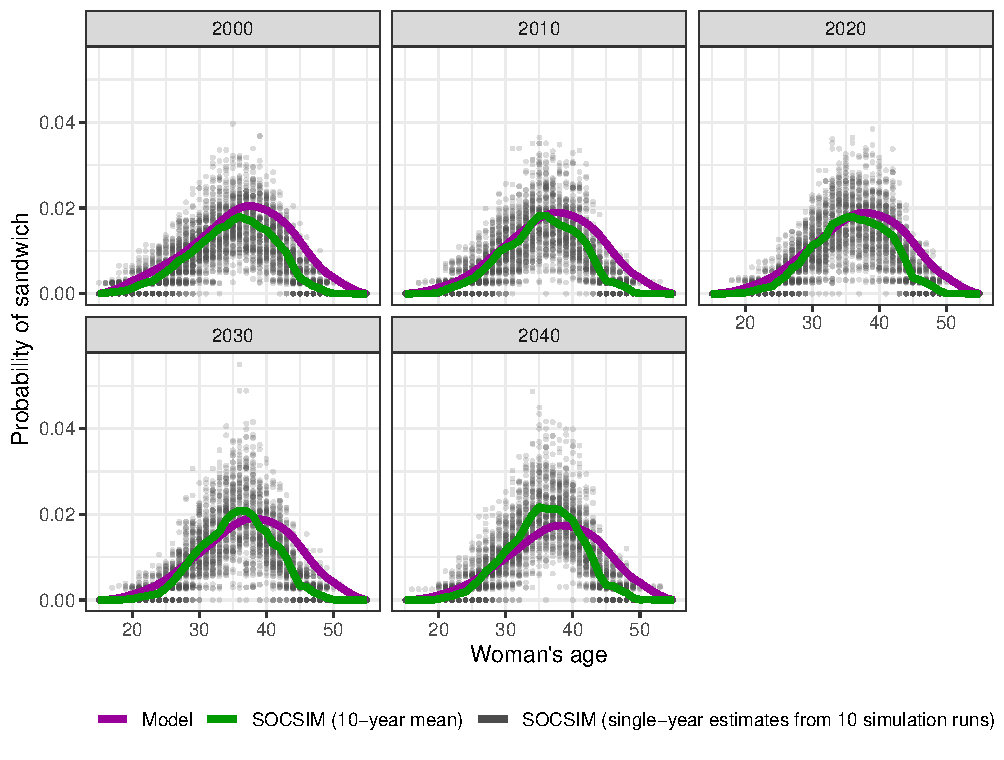
\includegraphics[width=3.64583in,height=\textheight]{resources/sandwich_comparative_USA}
\caption{Expected number of child deaths in the USA}
\end{figure}

\end{frame}

\begin{frame}{Make yourself heard!}
\protect\hypertarget{make-yourself-heard}{}


\includegraphics[width=0.41667in,height=\textheight]{resources/loud.png}

\begin{enumerate}
\tightlist
\item
  Brainstorming on project ideas?
\item
  How does all of this relate to your interests?
\item
  Final thoughts?
\end{enumerate}

\end{frame}

\end{document}
